\chapter{Introduction} \label{introduction}

\section{Motivation}
According to the International Data Corporation, the size of global data is expected to grow from 33 in 2018 to 175 zetabytes in 2025 as shown in Figure \ref{fig:data_growth}. \cite{IDS} To put that into perspective, the variations in one human genome can be compressed in a lossless fashion to 4 megabytes of data \cite{genome_size}, so the size of our data in 2025 will be equivalent to the digital representation of over 4 quadrillion humans. 

\begin{figure}[h]
\centering
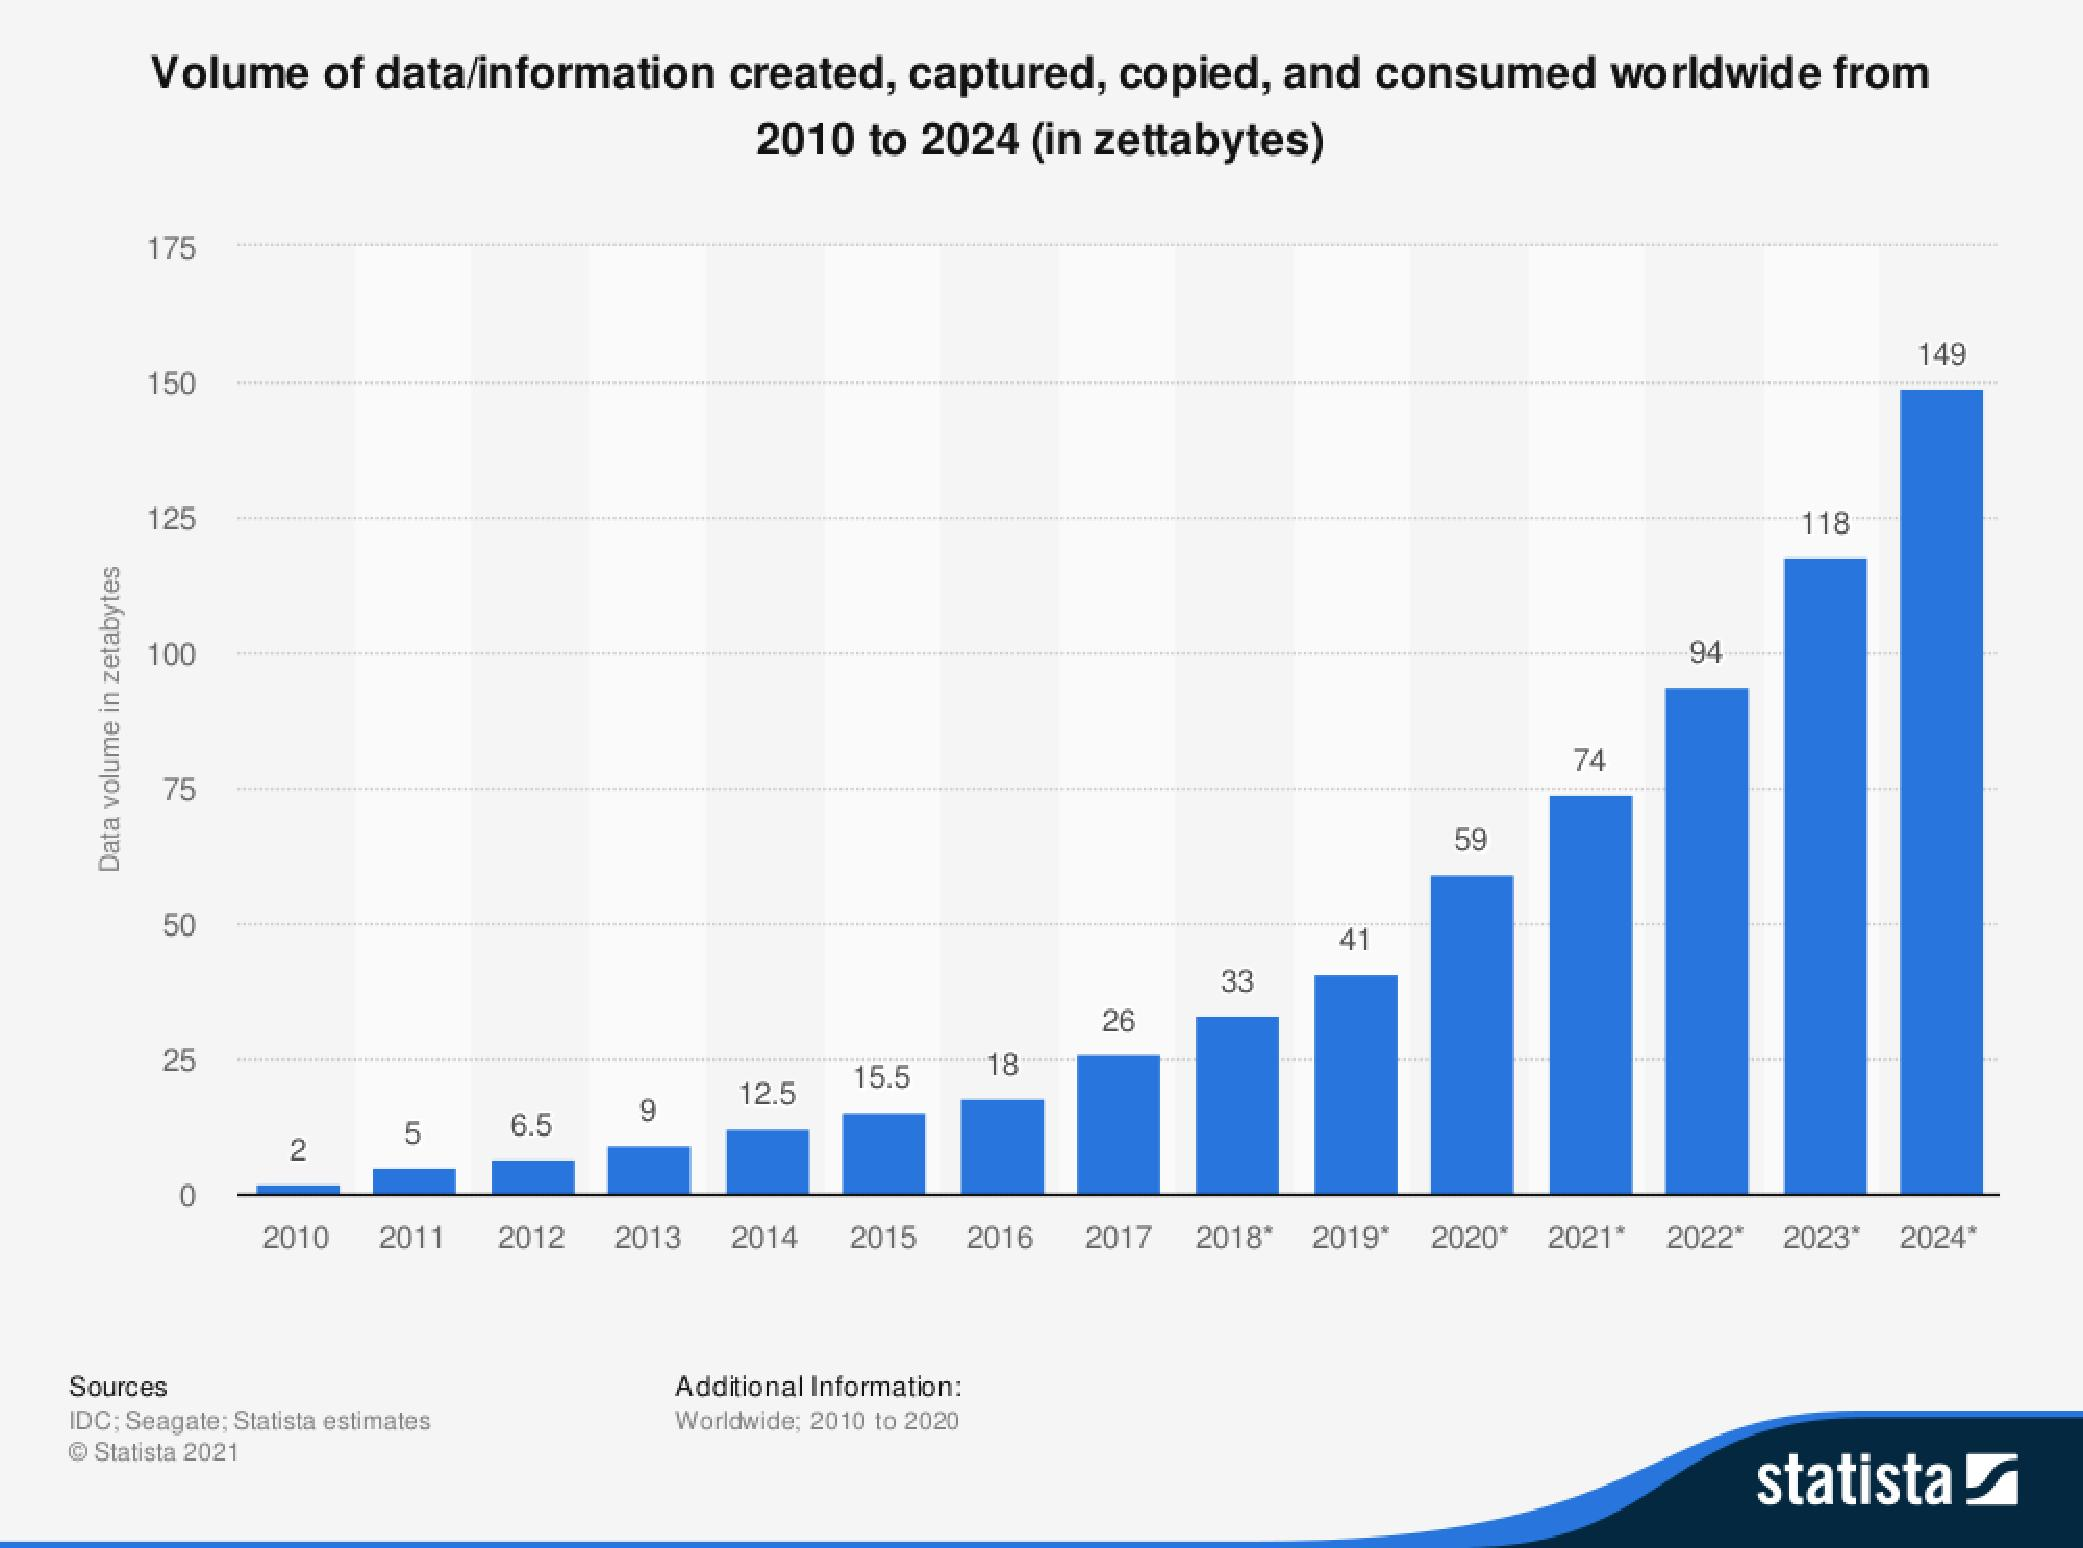
\includegraphics[width=0.5\textwidth]{Figures/global_data_growth.jpg}
\caption{Global Data Growth through 2024. Source: International Data Corporation}
\label{fig:data_growth}
\end{figure}

Along with all of this growth in data comes a growth in the amount of memory with which applications must work. In high performance computing (HPC), we define a computing cluster as a co-located set of computers, each individually called a node, configured for accomplishing a shared task.  Administrators have begun to include "big memory" nodes in these clusters which contain an above average amount of Random Access Memory (RAM) in order to address workloads that require excessive in-memory data. Prominent examples of these workloads include applications that utilize in-memory databases, graph analytics \cite{virtual_memory_tlb}, and large simulations. 

C++ is one of the most popular languages for distributed computing solutions, partly owing owing to the fact that it offers support for useful object-oriented abstractions in conjunction with highly optimized code. \cite{towards_dist_cpp} While much prior work has been dedicated to creating distributed libraries in C++ in \cite{STAPL}  \cite{practical_dist_c}
\cite{taskflow} \cite{intel_tbb} \cite{parallel_programming_w_charm} \cite{chapel} \cite{X10}, other separate work has attempted to improve performance on big memory applications through various optimizations \cite{virtual_memory_tlb}, and still other work has been dedicated to efficiently managing distributed memory \cite{spark} \cite{zookeeper} \cite{memcached} \cite{GAM}  few, if any, attempts have been made to create a library of standard data structures that are designed with big memory capabilities and work loads in mind. Additionally, few general purpose distributed computing libraries are available to the public under open source distribution licenses, as many provide some sort of proprietary value add. This research will be an attempt to create such an open source distributed computing library optimized for big memory utilization, experimenting with novel implementation techniques for standard data structures and drawing from existing literature when necessary. 

The main difference between PC2L and similar libraries will be in its focus on memory intensive workloads. Existing parallel and distributed libraries put more emphasis on optimizing the performance of single threads, This is perfectly fine for appplications in which there is more demand for CPU operations than memory bandwidth, but focusing entirely on the performance of individual threads can paradoxically lead to worse performance when memory footprint is a program's main constraint. PC2L will also be a library that can be included in any existing distributed C++ project instead of a stand-alone dialect of C++.    
\section{Contributions}
This thesis project will make the following contributions:
    \begin{itemize}
        \item an improved C++ memory allocator designed for effictively utilizing big memory
        \item Modular distributed data structures that can easily be inserted into existing programs with little change in code complexity 
            \begin{itemize}
                \item vector
                \item unordered multi-map
                \item graph
            \end{itemize}
        \item garbage collector designed for memory hungry programs running on distributed systems
    \end{itemize}
These contributions will be delivered through a portable C++ library that can run on both local computers and networked supercomputing clusters. 
